\subsection{Measure \& Sketch}
\subsubsection{Vorstellung}
Die App \emph{Measure \& Sketch} wird von \emph{SameBits} entwickelt.
Zur Zeit des Downloads (20. Januar 2018) ist die Applikation laut Google Play-Store auf zwischen $100.000$ und $500.000$ Android-Geräten installiert.
Auch diese Applikation ist unter der Kategorie ``Effizienz'' gelistet, und wird vom Entwickler mit den folgenden Worten beschrieben \citep{BitsMS}:

\begin{quote}
  ``Die Must-Have Zeichenapp für alle echten Ingenieure, Architekten, Bauarbeiter, Immobilienmakler, Handwerker wund [sic] natürlich für alle Heimwerker!''
\end{quote}

\noindent
Beim initialen Start der App wird der Benutzer mit Hilfe eines Overlays auf die möglichen Aktionen, die er in diesem Zustand tätigen kann, hingewiesen.
Hier bietet sich die Option zwischen den bestehenden Projekten zu wechseln, oder ein Neues anzulegen.
Über den Knopf ``Neu'' (siehe \autoref{fig:msmenu} kann der Nutzer ein neues Bild aufnehmen, oder direkt eines aus der Galerie importieren. \\

\begin{figure}[h]
  \centering
	\begin{subfigure}[b]{0.4\textwidth}
		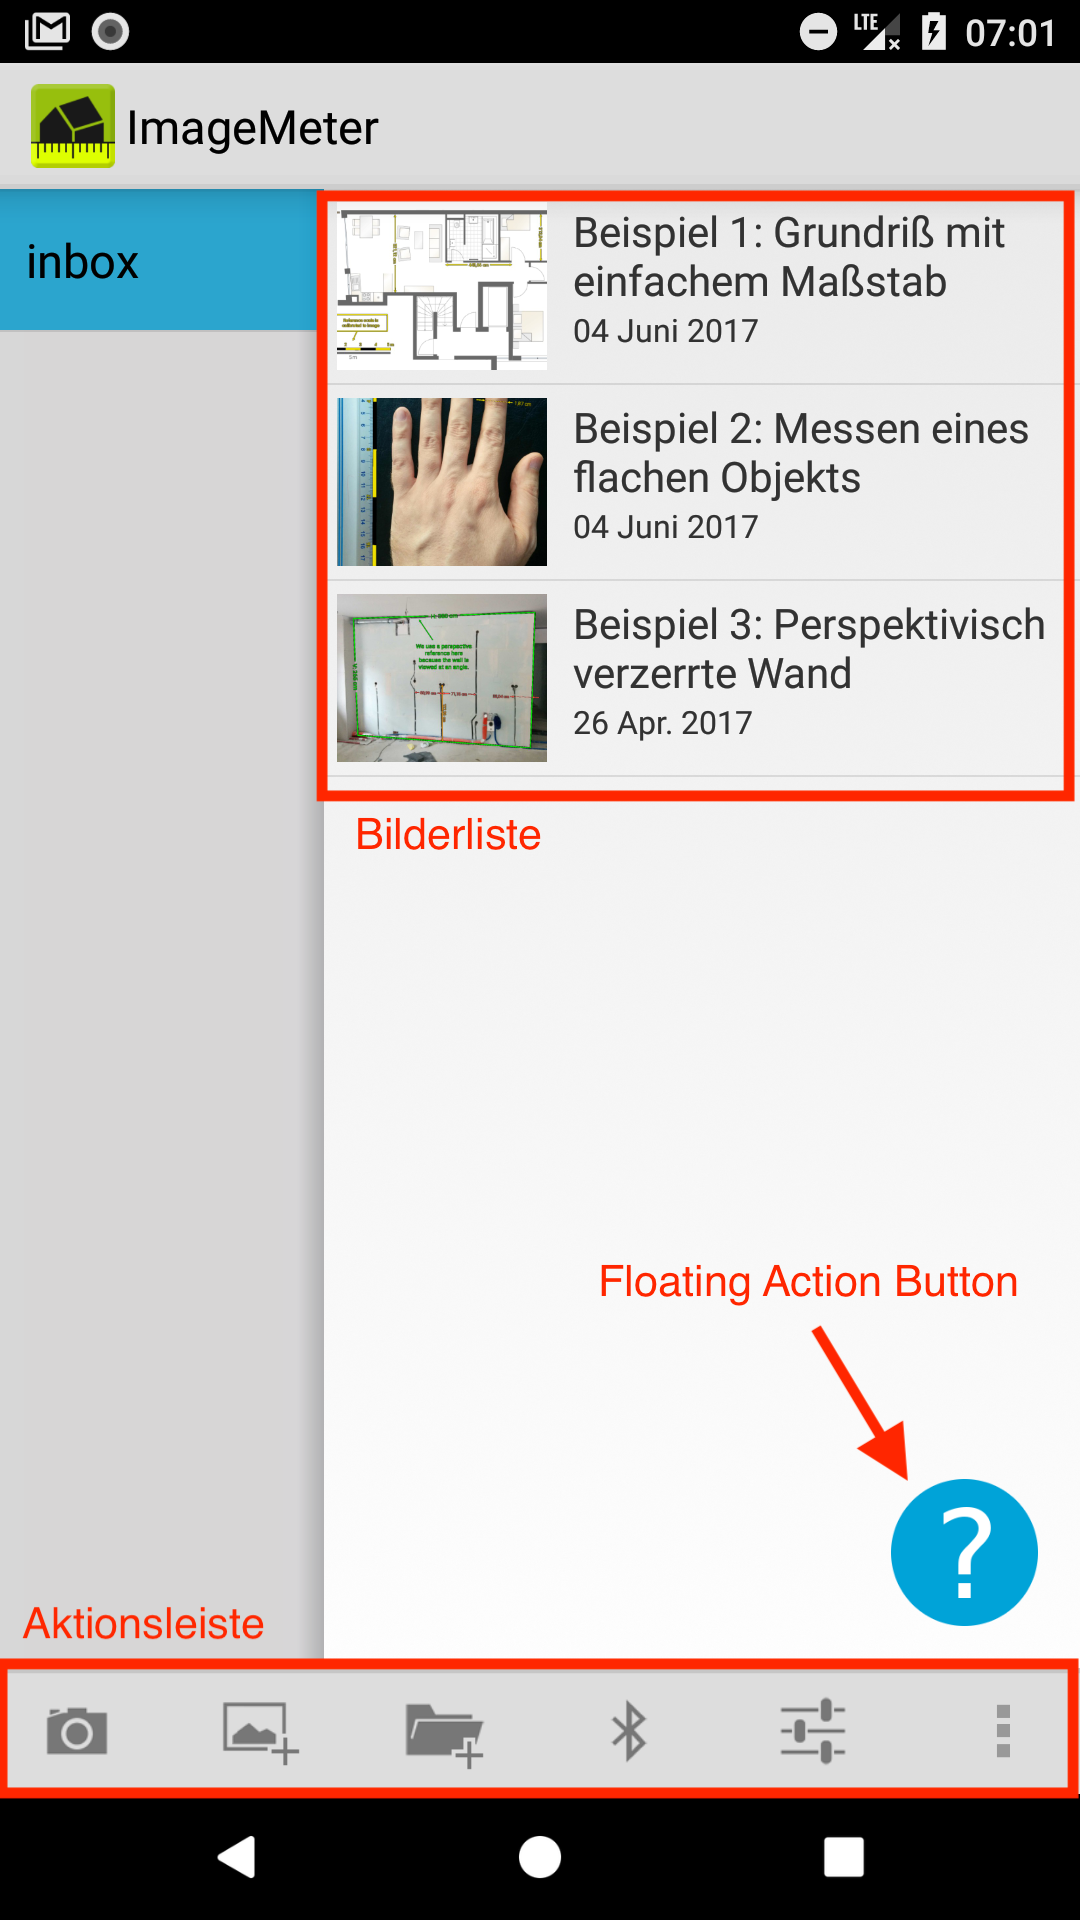
\includegraphics[keepaspectratio]{measure_sketch/menu}
		\caption{Startbildschirm}
		\label{fig:msmenu}	
	\end{subfigure}
	\begin{subfigure}[b]{0.4\textwidth}
		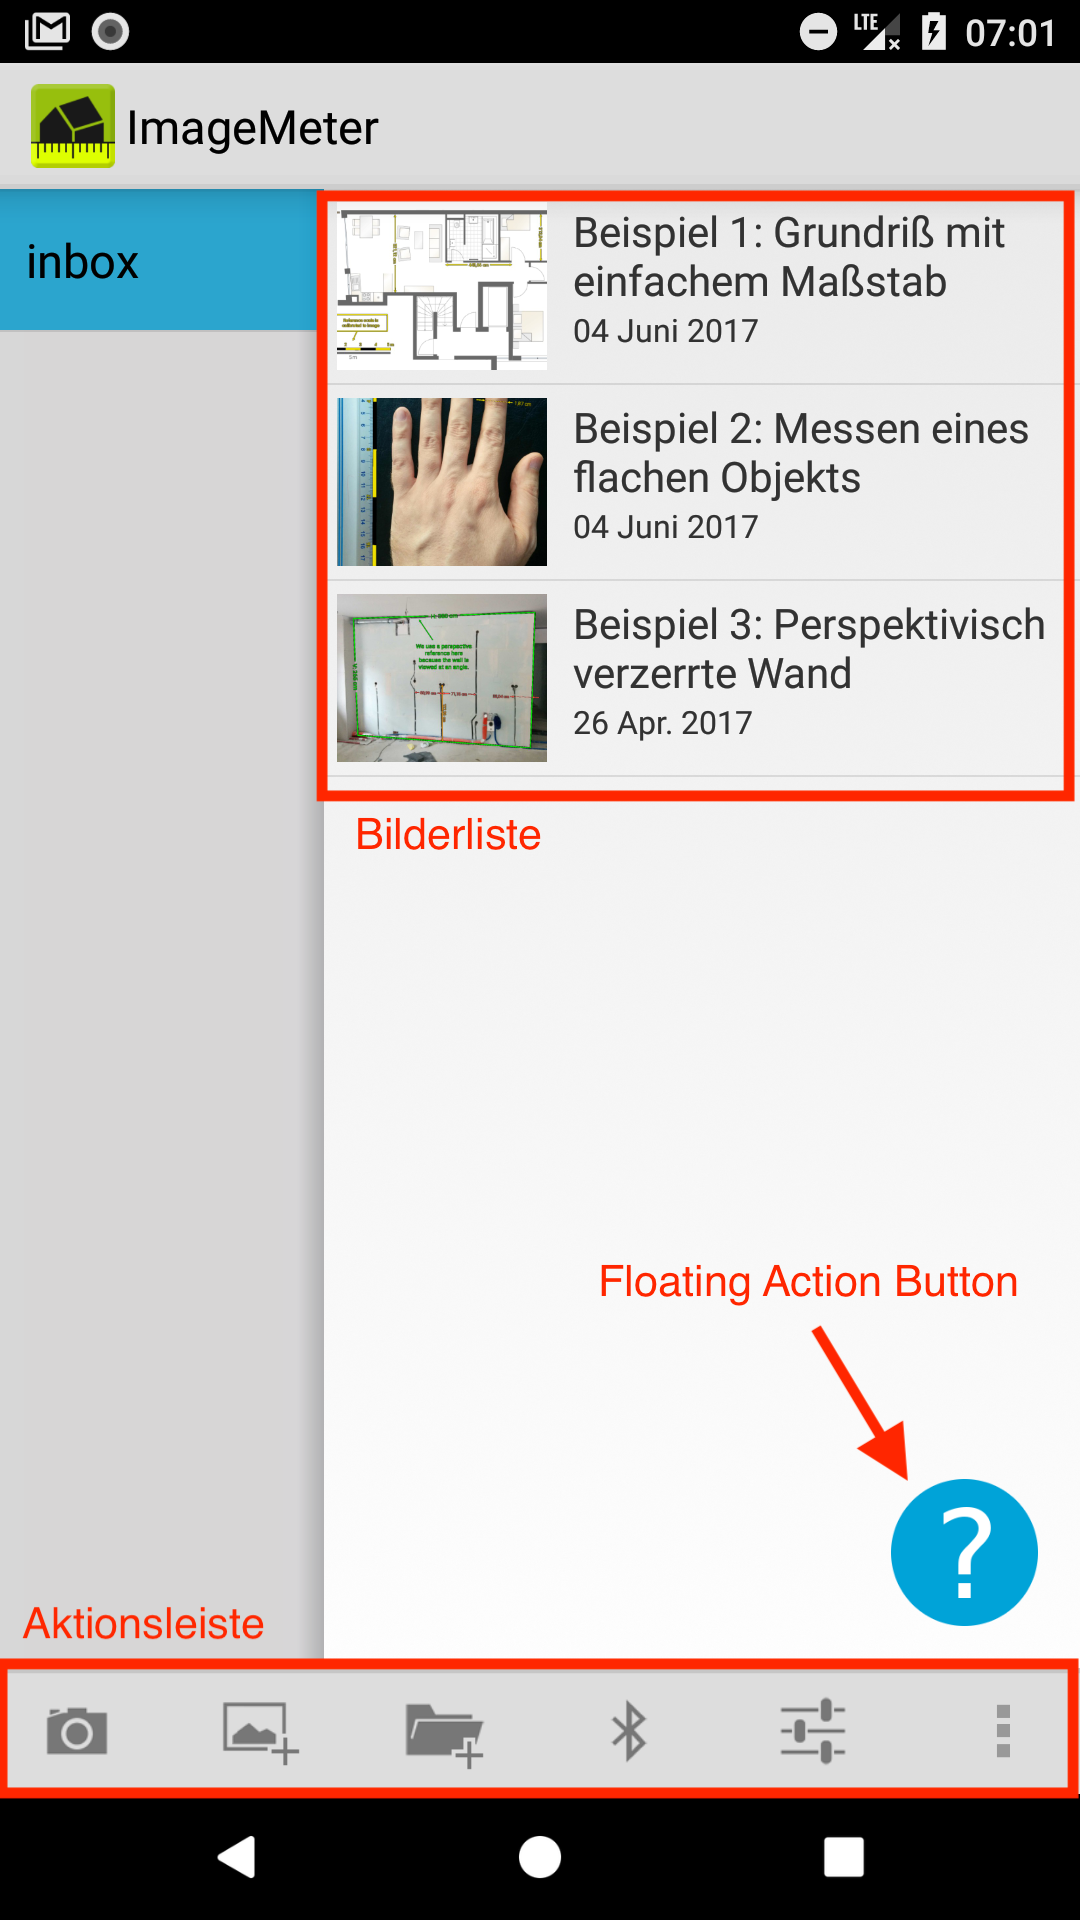
\includegraphics[keepaspectratio]{measure_sketch/menu}
		\caption{Aufmaße-Funktion} 
		\label{fig:msbar}	
	\end{subfigure}
  \caption{Measure \& Sketch beim Start der App und in der Aufmaße-Funktion}
\end{figure}

\noindent
\todo{Bilder mit Overlay}
Sobald man ein Bild ausgewählt hat, öffnet sich eine neue Benutzeröberfläche, in der, wie schon beim Start der App, durch ein Overlay alle möglichen Aktionen beschrieben werden (siehe \autoref{fig:msbar}).
In dieser Ansicht kann man das Bild mit drei verschiedenen Formen (Linie, Winkel, Freitext) annotieren. 
Zusätzlich können eingezeichnete Formen mit Messwerten beschriftet werden.\\

Weiterhin bietet sich die Gelegenheit, das bearbeitete Bild zur Galerie, \emph{Evernote} oder Universal \todo{gucken was gemeint ist} zu exportieren, oder direkt per E-Mail zu verschicken.
Auch bei dieser App kann man modifizierte Bilder speichern, und zu einem späteren Zeitpunkt zur Weiterverarbeitung wieder öffnen. \\

\subsubsection{Evaluation}

\begin{wrapfigure}{R}{0.4\textwidth}
	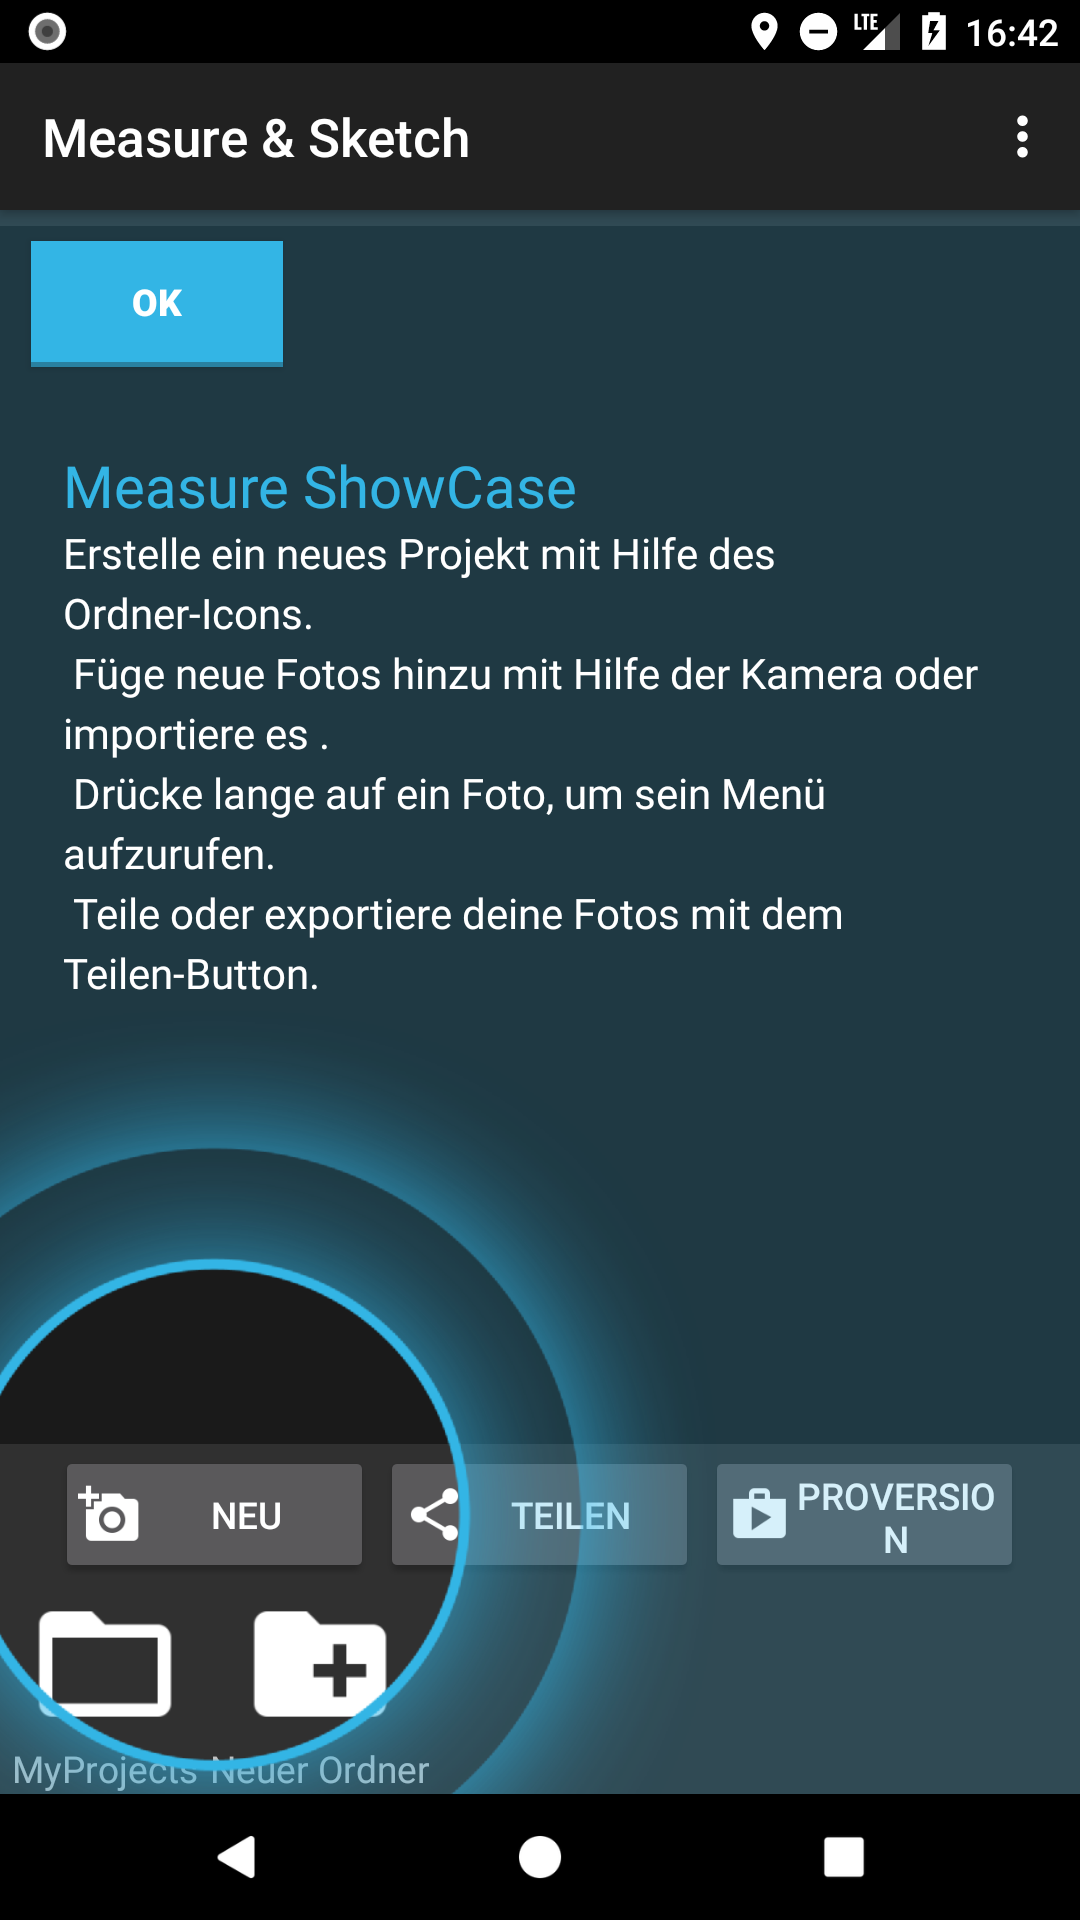
\includegraphics[keepaspectratio, width=0.4\textwidth]{measure_sketch/help_start}
	\caption{Hilfe-Overlay}
	\label{fig:mshelp}
\end{wrapfigure}

Auch diese App bedient sich eines Hilfe-Overlays beim ersten Start, überfordert den Benutzer jedoch mit zu viel Text. So erfüllt dieses Tooltip ihre Funktion als Hilfestellung nicht, sondern überfordert den Nutzer mit Text. Alternativ bietet sich auch bei dieser App wie in \autoref{fig:pmhelp} mit Icons zu arbeiten, sodass die Gedächtnisbelastung minimiert wird. \\

Die App kann als negativ-Beispiel bezüglich der Nielsen-Heuristiken betrachtet werden. Es gibt weder Undo- oder Redo-Button, noch wird in irgendeiner Weise hervorgehoben, welche Form aktuell ausgewählt ist. Dies führte beim Löschen oft zu Überraschungen. \\

 Außerdem unterstützt die App keinerlei Gesten zur Navigation im Bild. So lässt sich der abgebildete Bereich des Bildes weder zoomen, noch kann der Benutzer das Bild rotieren oder verschieben. Um Formen zu zeichnen bedient sich die App eine für den Benutzer unnatürliche Geste, denn hierzu muss der Nutzer gleichzeitig mit zwei Fingern die Form in die beiden gewünschten Richtungen ``aufziehen''. So fühlt sich der Zeichen-Prozess nicht nur unnatürlich an, sondern ist in der Größe der Form durch die Spannweite der Finger des Benutzers beschränkt. \\
 
 Zusätzlich schließt dies die Benutzung der App mit einer Hand aus, was Nielsen~\autoref{itm:16} klar widerspricht. Als Bildschirmausrichtung wird nur der Portrait-Modus unterstützt, was gerade die Bearbeitung von im Landscape aufgenommenen Bildern zu einer Herausforderung macht. \\

